%% ============================================================
%%  Chapter 4 — Results
%% ============================================================
\chapter{Results}
\label{ch:results}

This chapter reports quantitative outcomes from four sets of experiments:
(1) SEDM cross-intent evaluation,
(2) per-intent action distribution analysis,
(3) composite risk and escalation risk characterisation, and
(4) DQN training dynamics.
All results were obtained using the protocols and hyperparameters described
in Chapter~\ref{ch:methodology}.

%% ── 4.1 SEDM Cross-Intent Evaluation ────────────────────────
\section{SEDM Cross-Intent Evaluation}
\label{sec:results_sedm}

\subsection{Overall Performance Summary}

Table~\ref{tab:eval_summary} summarises SEDM performance across all four
attacker intents, evaluated over 30 episodes of 200 steps each.
The SEDM achieves detection rates exceeding 99\% across all four profiles,
demonstrating robust and consistent threat coverage without any
intent-specific training or tuning.

\begin{table}[ht]
  \centering
  \caption{SEDM evaluation summary across all attacker intents
           (30 episodes $\times$ 200 steps each).
           Mean $\pm$ standard deviation are reported.}
  \label{tab:eval_summary}
  \begin{tabular}{lcccccc}
    \toprule
    Intent & Mean Reward & Std Reward & Det.\ Rate & FP Rate & Avg Threat & Avg Risk \\
    \midrule
    STEALTHY      & 1012.22 & 51.37 & \textbf{99.09\%} & 35.56\% & 0.806 & 0.632 \\
    AGGRESSIVE    & 1090.84 & 19.80 & \textbf{99.47\%} &  6.67\% & 0.854 & 0.709 \\
    TARGETED      & 1127.10 & 20.98 & \textbf{99.48\%} &  3.33\% & 0.853 & 0.673 \\
    OPPORTUNISTIC &  896.05 & 32.98 & \textbf{99.41\%} & 15.00\% & 0.790 & 0.663 \\
    \bottomrule
  \end{tabular}
\end{table}

\subsection{Detection Rate Analysis}

Detection rates are uniformly high across all four intent profiles,
ranging from 99.09\% (STEALTHY) to 99.48\% (TARGETED).
The 0.39 percentage-point spread across profiles is remarkably small,
indicating that the SEDM's intent-aware escalation risk computation
successfully adapts to the structural differences between attack campaigns.

Under the STEALTHY intent, the campaign proceeds slowly through early kill
chain stages with low escalation risk.
The SEDM assigns Low-band actions (ALLOW, LOG) at early stages, correctly
identifying benign-like reconnaissance.
When STEALTHY campaigns eventually progress to later stages (Installation,
C2), the escalation risk increases, and the SEDM appropriately escalates
to BLOCK/ALERT.
The small number of missed detections (0.91\%) corresponds to RECONNAISSANCE
steps where the attacker generates NORMAL-type traffic (triggering R1 $\to$
ALLOW) but the ground-truth label is technically an attack.

The TARGETED intent, which follows a focused exploitation chain, achieves
the highest detection rate (99.48\%) because the direct EXPLOITATION $\to$
INSTALLATION $\to$ C2 path consistently falls in the High escalation risk
band across all stages.
The matrix lookup always returns BLOCK or ALERT for this path, and no false
negatives arise on genuine attack steps.

\subsection{False Positive Rate Analysis}

False positive rates vary substantially across intents: 3.33\% (TARGETED),
6.67\% (AGGRESSIVE), 15.00\% (OPPORTUNISTIC), and 35.56\% (STEALTHY).
This variation reflects a fundamental property of the SEDM's design: it
responds to kill chain stage and escalation risk, not to whether traffic
is technically benign.

The elevated false positive rate for STEALTHY (35.56\%) arises because
STEALTHY campaigns generate extended periods of low-severity attack traffic
(RECONNAISSANCE, ANALYSIS) that is distinguishable from benign traffic only
by the ground-truth label.
When the attacker sends FUZZERS or GENERIC at a low rate (true attack),
the SEDM may assign LOG or TROLL — a non-ALLOW action — counting as a
true positive for detection but not necessarily at the level a human
operator might expect.

The very low false positive rate for TARGETED (3.33\%) reflects the
concentrated nature of targeted campaigns: most steps involve high-severity
attack types at advanced kill chain stages, with few benign intermissions.
The SEDM rarely encounters a benign step under TARGETED, and when it does,
the escalation risk is typically Low (the focused attack path has few
backtrack opportunities), returning LOG rather than BLOCK/ALERT.

\subsection{Reward Distribution}

Mean episode rewards range from 896.05 (OPPORTUNISTIC) to 1127.10 (TARGETED).
The reward is determined by the alignment between the SEDM's actions and
the reward matrix (Table~\ref{tab:reward_matrix_meth}).

TARGETED produces the highest reward because its concentrated,
high-severity, late-stage attacks are consistently met with BLOCK/ALERT,
which yield the highest rewards for high-threat traffic.
Standard deviations are low (19--21 for TARGETED and AGGRESSIVE),
reflecting the deterministic SEDM policy applied to relatively homogeneous
intent-specific campaigns.

OPPORTUNISTIC yields the lowest mean reward (896.05) with higher standard
deviation (32.98).
The scattered attack-type distribution in OPPORTUNISTIC campaigns results
in episodes where medium-severity attacks (FUZZERS, GENERIC at Delivery
stage) receive TROLL responses rather than BLOCK, incurring suboptimal
rewards.
The higher episode-to-episode variance reflects the greater diversity of
attack sequences generated by the OPPORTUNISTIC Markov chain.

STEALTHY yields moderate mean reward (1012.22) with the highest standard
deviation (51.37), consistent with its inherently variable behaviour:
some STEALTHY episodes remain in early kill chain stages for extended
periods (producing many LOG/ALLOW rewards), while others escalate to
late stages (producing BLOCK/ALERT rewards).
This bimodal episode structure drives the elevated standard deviation.

\begin{figure}[ht]
  \centering
  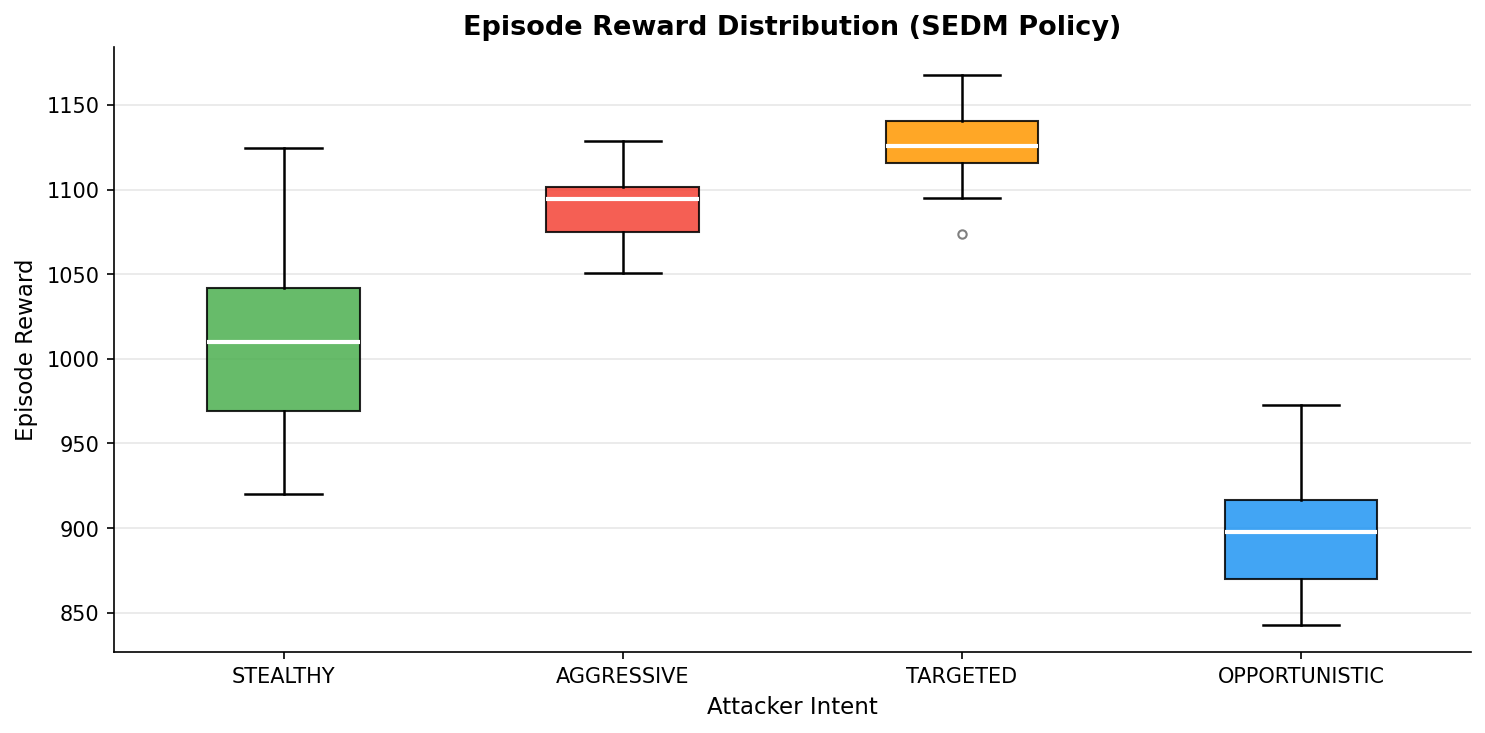
\includegraphics[width=0.82\textwidth]{figures/reward_boxplot}
  \caption{Episode reward distributions per attacker intent (30 episodes each).
           Boxes show the interquartile range; whiskers extend to 1.5$\times$IQR;
           circles indicate outliers.}
  \label{fig:reward_boxplot}
\end{figure}

%% ── 4.2 Action Distribution Analysis ────────────────────────
\section{Per-Intent Action Distribution}
\label{sec:results_action}

Table~\ref{tab:action_dist} reports the percentage of steps assigned to each
honeypot action across the four attacker intents.

\begin{table}[ht]
  \centering
  \caption{Action distribution across attacker intents (all 30 evaluation
           episodes pooled).
           Values are percentages of total steps.}
  \label{tab:action_dist}
  \begin{tabular}{lrrrrr}
    \toprule
    Intent & ALLOW & LOG & TROLL & BLOCK & ALERT \\
    \midrule
    STEALTHY      & 0.0\% & 1.1\% & 0.7\% & 17.9\% & 80.3\% \\
    AGGRESSIVE    & 0.0\% & 0.0\% & 0.0\% &  4.6\% & 95.4\% \\
    TARGETED      & 0.0\% & 0.5\% & 0.1\% &  5.4\% & 94.0\% \\
    OPPORTUNISTIC & 0.1\% & 1.0\% & 0.4\% & 24.6\% & 73.8\% \\
    \bottomrule
  \end{tabular}
\end{table}

\subsection{Dominance of ALERT and BLOCK}

ALERT and BLOCK together account for 98.2--100\% of actions across all
intent profiles.
This is consistent with the evaluation scenarios: all four intents involve
continuous attack traffic with no extended benign periods, keeping the
threat level elevated and the kill chain stage at advanced positions.

The near-total absence of ALLOW (0.0--0.1\%) confirms that the SEDM correctly
avoids passthrough for ongoing attack campaigns.
The R1 override (NORMAL traffic $\to$ ALLOW) fires only for the 0.1\%
of OPPORTUNISTIC steps that generate true NORMAL-type traffic.

\subsection{AGGRESSIVE and TARGETED: ALERT-Dominated}

AGGRESSIVE (95.4\% ALERT) and TARGETED (94.0\% ALERT) are dominated by
ALERT responses.
Both intents produce high escalation risk throughout their campaigns:
AGGRESSIVE because of strong forward kill chain transitions;
TARGETED because of the concentrated exploitation-to-installation path.
High escalation risk places most stages in the High band, mapping to
ALERT at Installation, C2, and Actions on Objectives (Table~\ref{tab:sedm_matrix}).

The R2 override (DOS/WORMS $\to$ upgrade) further increases ALERT frequency
for AGGRESSIVE campaigns, which generate significant DOS and WORMS traffic.

\subsection{STEALTHY: Mixed BLOCK and ALERT}

The STEALTHY distribution shows a more balanced profile: 80.3\% ALERT and
17.9\% BLOCK.
STEALTHY campaigns generate significant BACKDOORS traffic (Installation stage,
Medium escalation risk under Stealthy intent), which maps to BLOCK rather
than ALERT (SEDM[4][1] = BLOCK).
The resulting BLOCK actions represent 17.9\% of steps, substantially more
than in any other intent.

The LOG and TROLL fractions (1.1\% and 0.7\%) correspond to early-stage
STEALTHY steps where the attacker is in RECONNAISSANCE or WEAPONIZATION with
Low-to-Medium escalation risk.
These provide the opportunity for intelligence gathering before the campaign
escalates.

\subsection{OPPORTUNISTIC: Distributed Across BLOCK and ALERT}

OPPORTUNISTIC yields a more balanced split between BLOCK (24.6\%) and
ALERT (73.8\%).
The scattered attack-type distribution means that FUZZERS and GENERIC attacks
at DELIVERY stage (Medium escalation risk under OPPORTUNISTIC intent)
frequently map to TROLL or BLOCK rather than ALERT, producing the higher
BLOCK fraction compared to AGGRESSIVE and TARGETED.

\begin{figure}[ht]
  \centering
  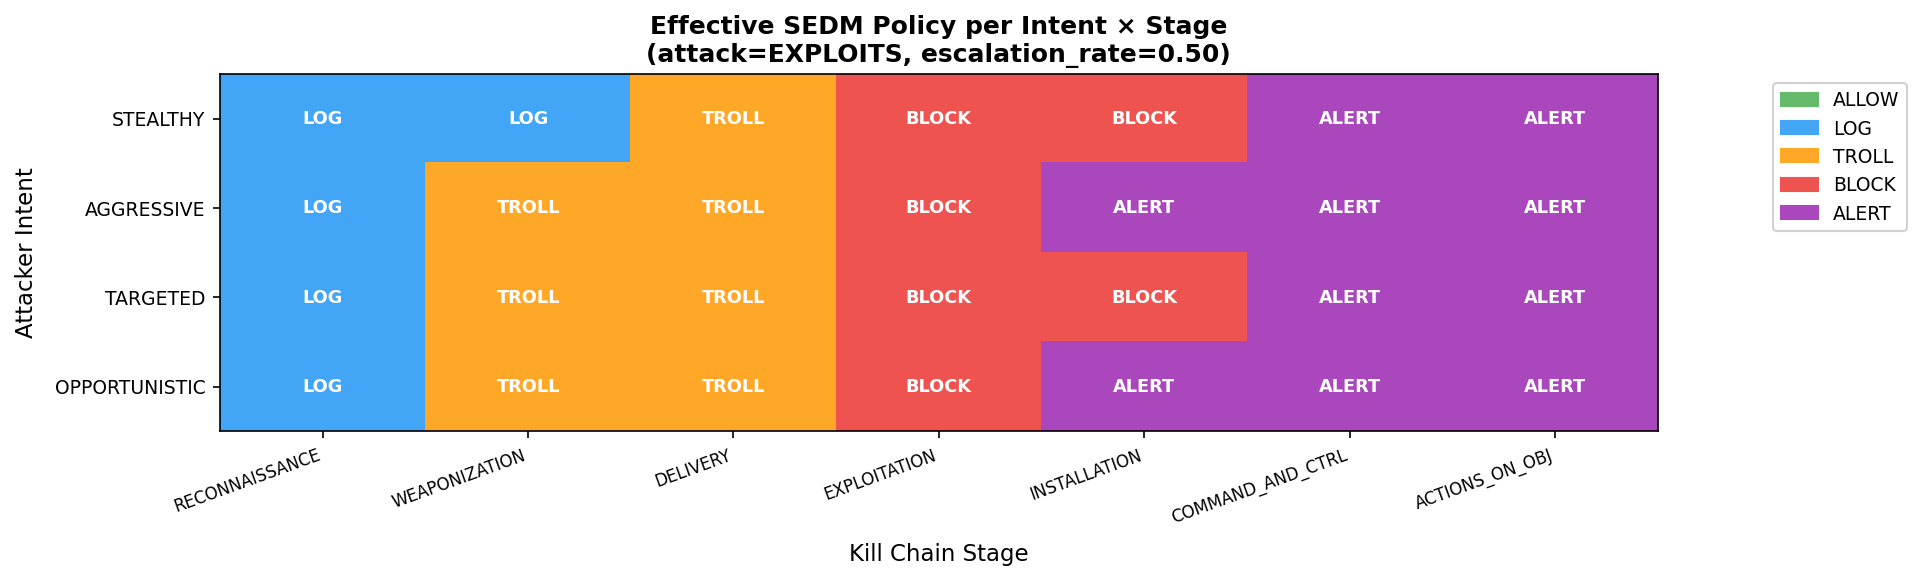
\includegraphics[width=0.90\textwidth]{figures/effective_policy_per_intent}
  \caption{Stacked bar chart of action distribution across the four attacker
           intents. Each bar represents 30 pooled evaluation episodes
           (6\,000 steps total per intent).}
  \label{fig:action_dist}
\end{figure}

%% ── 4.3 Composite Risk Characterisation ──────────────────────
\section{Escalation and Composite Risk Analysis}
\label{sec:results_risk}

\subsection{Composite Risk Score Distribution}

The composite risk score $\rho_c$ (Equation~\ref{eq:composite_risk}) provides
an aggregate threat index at each step.
Mean composite risk scores range from 0.632 (STEALTHY) to 0.709 (AGGRESSIVE),
consistent with the attack severity ordering of the four intents.

AGGRESSIVE campaigns achieve the highest mean composite risk (0.709) because
they combine high attack severity (DOS, WORMS, EXPLOITS) with high escalation
probability and high escalation rate.
STEALTHY campaigns have the lowest mean composite risk (0.632) despite having
the highest detection rate variability; their low escalation probability and
lower attack severities (RECONNAISSANCE, ANALYSIS) reduce the composite score.

\begin{figure}[ht]
  \centering
  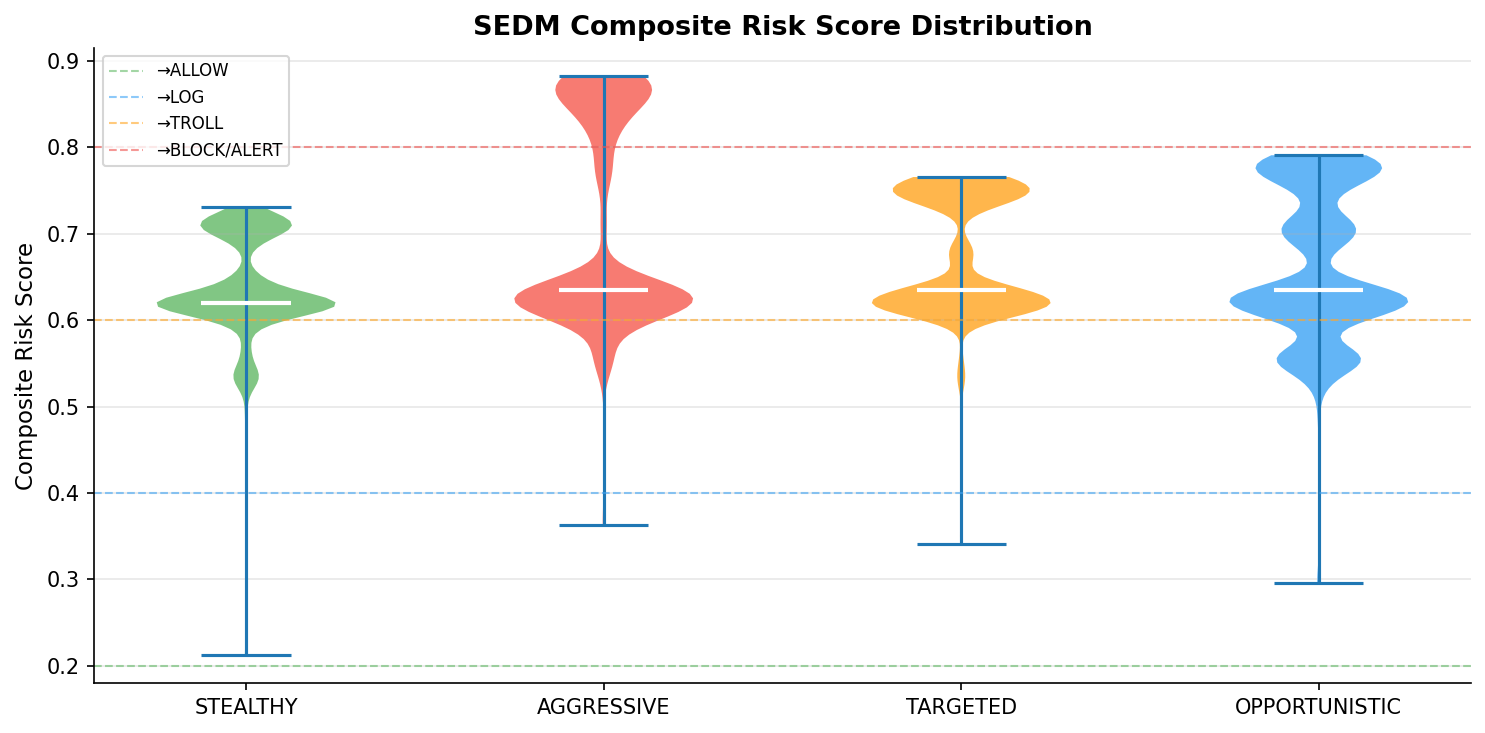
\includegraphics[width=0.82\textwidth]{figures/composite_risk_distribution}
  \caption{Distribution of composite risk scores across all evaluation
           steps, stratified by attacker intent.
           Higher risk scores correspond to more dangerous attack configurations.}
  \label{fig:composite_risk}
\end{figure}

\subsection{Escalation Risk by Kill Chain Stage}

Figure~\ref{fig:esc_risk_per_intent} shows the escalation risk $\rho(k, \pi)$
as a function of kill chain stage for each intent profile.
The values are computed analytically from the intent-specific Markov
transition matrices.

Several patterns are noteworthy:
%
\begin{itemize}
  \item For AGGRESSIVE, escalation risk is consistently high ($>0.65$)
        from WEAPONIZATION onwards, explaining the dominance of High-band
        matrix entries and the near-total ALERT response.
  \item For STEALTHY, escalation risk is low ($<0.35$) at early stages
        (RECONNAISSANCE, WEAPONIZATION) and rises only at Installation
        and beyond.
        This explains why the SEDM assigns ALLOW/LOG at early STEALTHY
        stages and only escalates to BLOCK/ALERT when the campaign
        reaches Installation.
  \item For TARGETED, escalation risk is high from EXPLOITATION onwards,
        consistent with the focused exploitation chain.
        Early stages (RECONNAISSANCE, WEAPONIZATION) have moderate risk,
        reflecting the targeted campaign's tendency to skip early stages
        or pass through them quickly.
  \item For OPPORTUNISTIC, escalation risk is moderate ($0.35$--$0.65$)
        across most stages, placing many steps in the Medium band.
        This drives the significant BLOCK fraction (24.6\%) as Medium-band
        EXPLOITATION steps map to BLOCK.
\end{itemize}

\begin{figure}[ht]
  \centering
  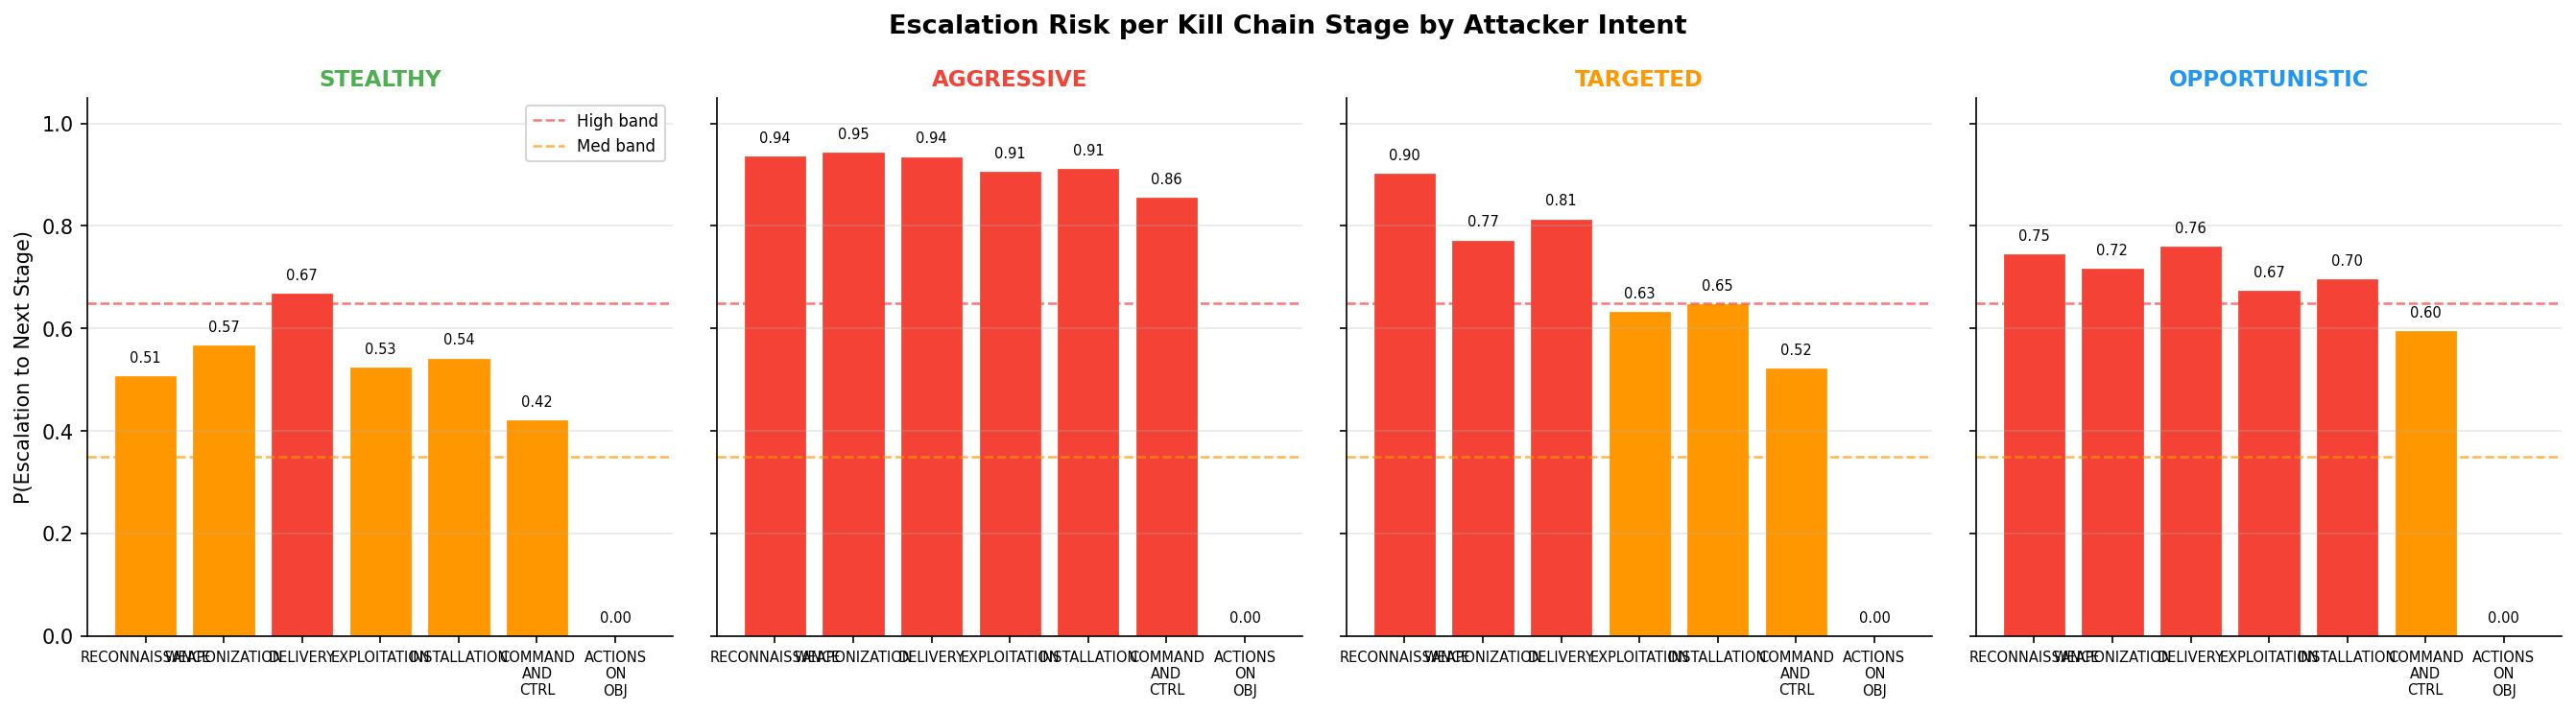
\includegraphics[width=0.90\textwidth]{figures/escalation_risk_per_intent}
  \caption{Escalation risk $\rho(k, \pi)$ as a function of kill chain stage,
           for all four attacker intent profiles.
           Dashed horizontal lines show the Low (0.35) and High (0.65)
           band thresholds.}
  \label{fig:esc_risk_per_intent}
\end{figure}

\subsection{SEDM Decision Matrix Visualisation}

Figure~\ref{fig:sedm_heatmap} shows a colour-coded representation of
the $7 \times 3$ SEDM, with action severity encoded on a five-point
colour scale (ALLOW = lightest, ALERT = darkest).
The clear escalation gradient from top-left (Reconnaissance/Low = ALLOW)
to bottom-right (Actions on Objectives/High = ALERT) confirms the
proportionality principle underlying the matrix design.

\begin{figure}[ht]
  \centering
  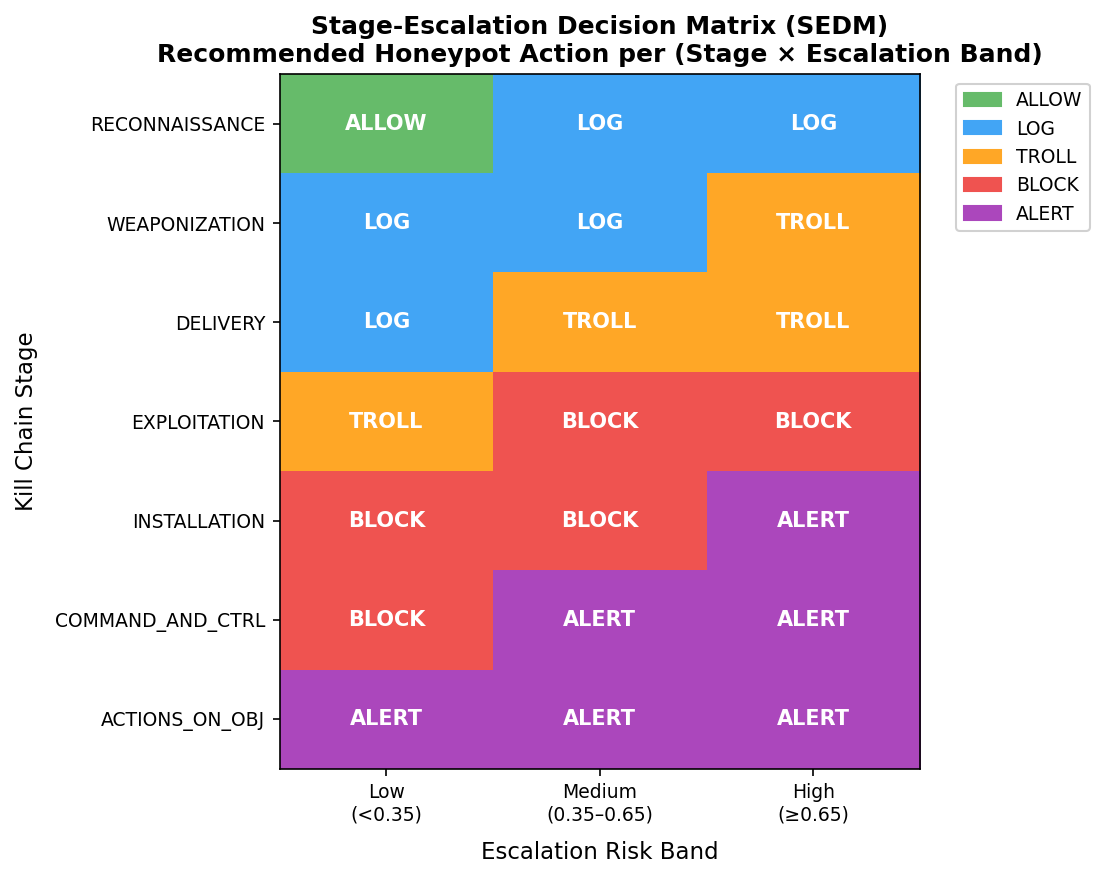
\includegraphics[width=0.65\textwidth]{figures/sedm_decision_matrix}
  \caption{Stage-Escalation Decision Matrix (SEDM) visualised as a
           colour-coded heatmap.
           Rows represent kill chain stages (Reconnaissance at top,
           Actions on Objectives at bottom);
           columns represent escalation risk bands
           (Low on left, High on right).}
  \label{fig:sedm_heatmap}
\end{figure}

%% ── 4.4 Kill Chain Stage Distribution ───────────────────────
\section{Kill Chain Stage Distribution}
\label{sec:results_killchain}

\begin{figure}[ht]
  \centering
  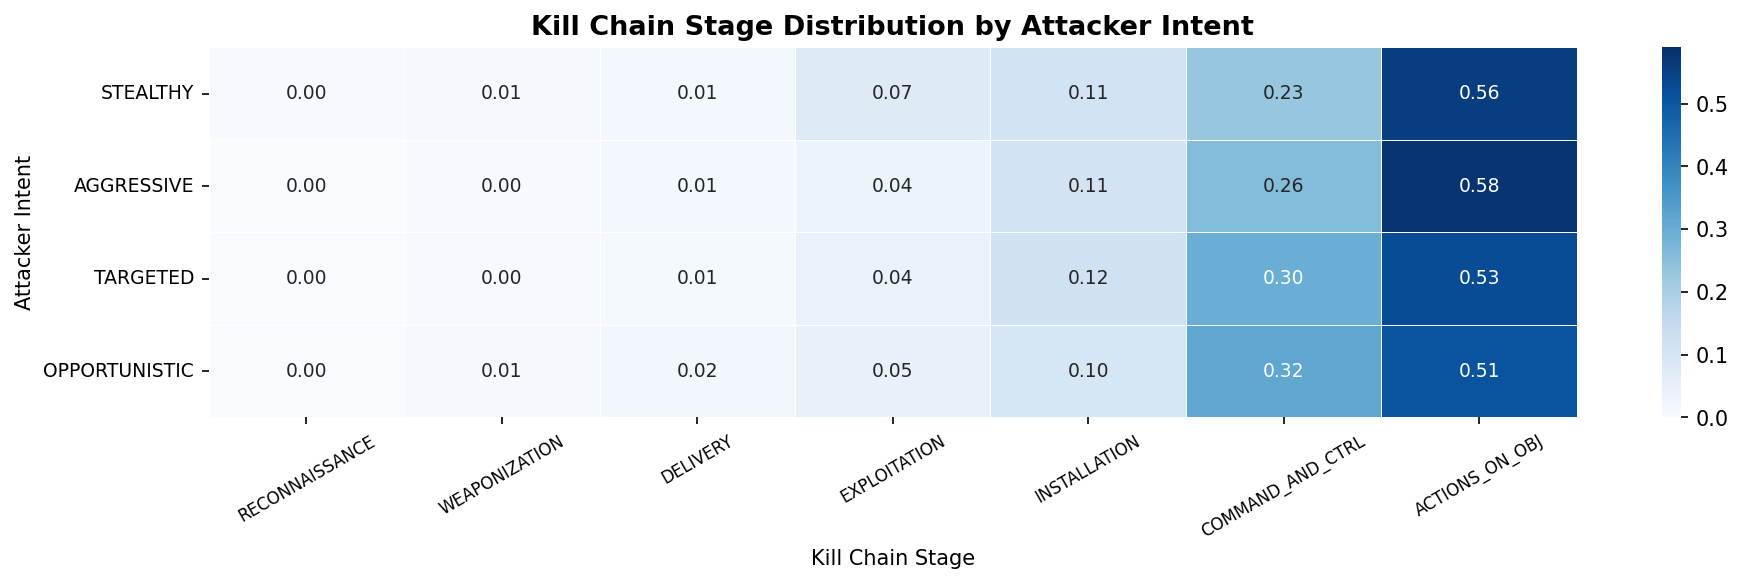
\includegraphics[width=0.88\textwidth]{figures/kill_chain_distribution}
  \caption{Distribution of kill chain stages visited across evaluation
           episodes, stratified by attacker intent.
           Bars show the fraction of steps in each stage.}
  \label{fig:killchain_dist}
\end{figure}

Figure~\ref{fig:killchain_dist} shows the kill chain stage distribution
across evaluation episodes for each intent.
The distributions are consistent with the intent descriptions in
Section~\ref{sec:intents}:
%
\begin{itemize}
  \item \textbf{STEALTHY}: overrepresented at RECONNAISSANCE and
        WEAPONIZATION; relatively rare at ACTIONS\_ON\_OBJ.
  \item \textbf{AGGRESSIVE}: concentrated at EXPLOITATION, INSTALLATION,
        and COMMAND\_AND\_CTRL; rapid progression means less time in
        early stages.
  \item \textbf{TARGETED}: concentrated at EXPLOITATION and INSTALLATION,
        consistent with the focused exploit chain.
  \item \textbf{OPPORTUNISTIC}: roughly uniform across mid-chain stages
        (DELIVERY through COMMAND\_AND\_CTRL), reflecting the scattered
        transition structure.
\end{itemize}

%% ── 4.5 DQN Training Dynamics ────────────────────────────────
\section{DQN Training Dynamics}
\label{sec:results_dqn}

\subsection{Overview}

The DQN baseline was trained for 300 episodes of 500 steps each on the
OPPORTUNISTIC intent.
Training metrics were logged to \texttt{logs/metrics.csv} and visualised
as six-panel training curves.

\begin{figure}[ht]
  \centering
  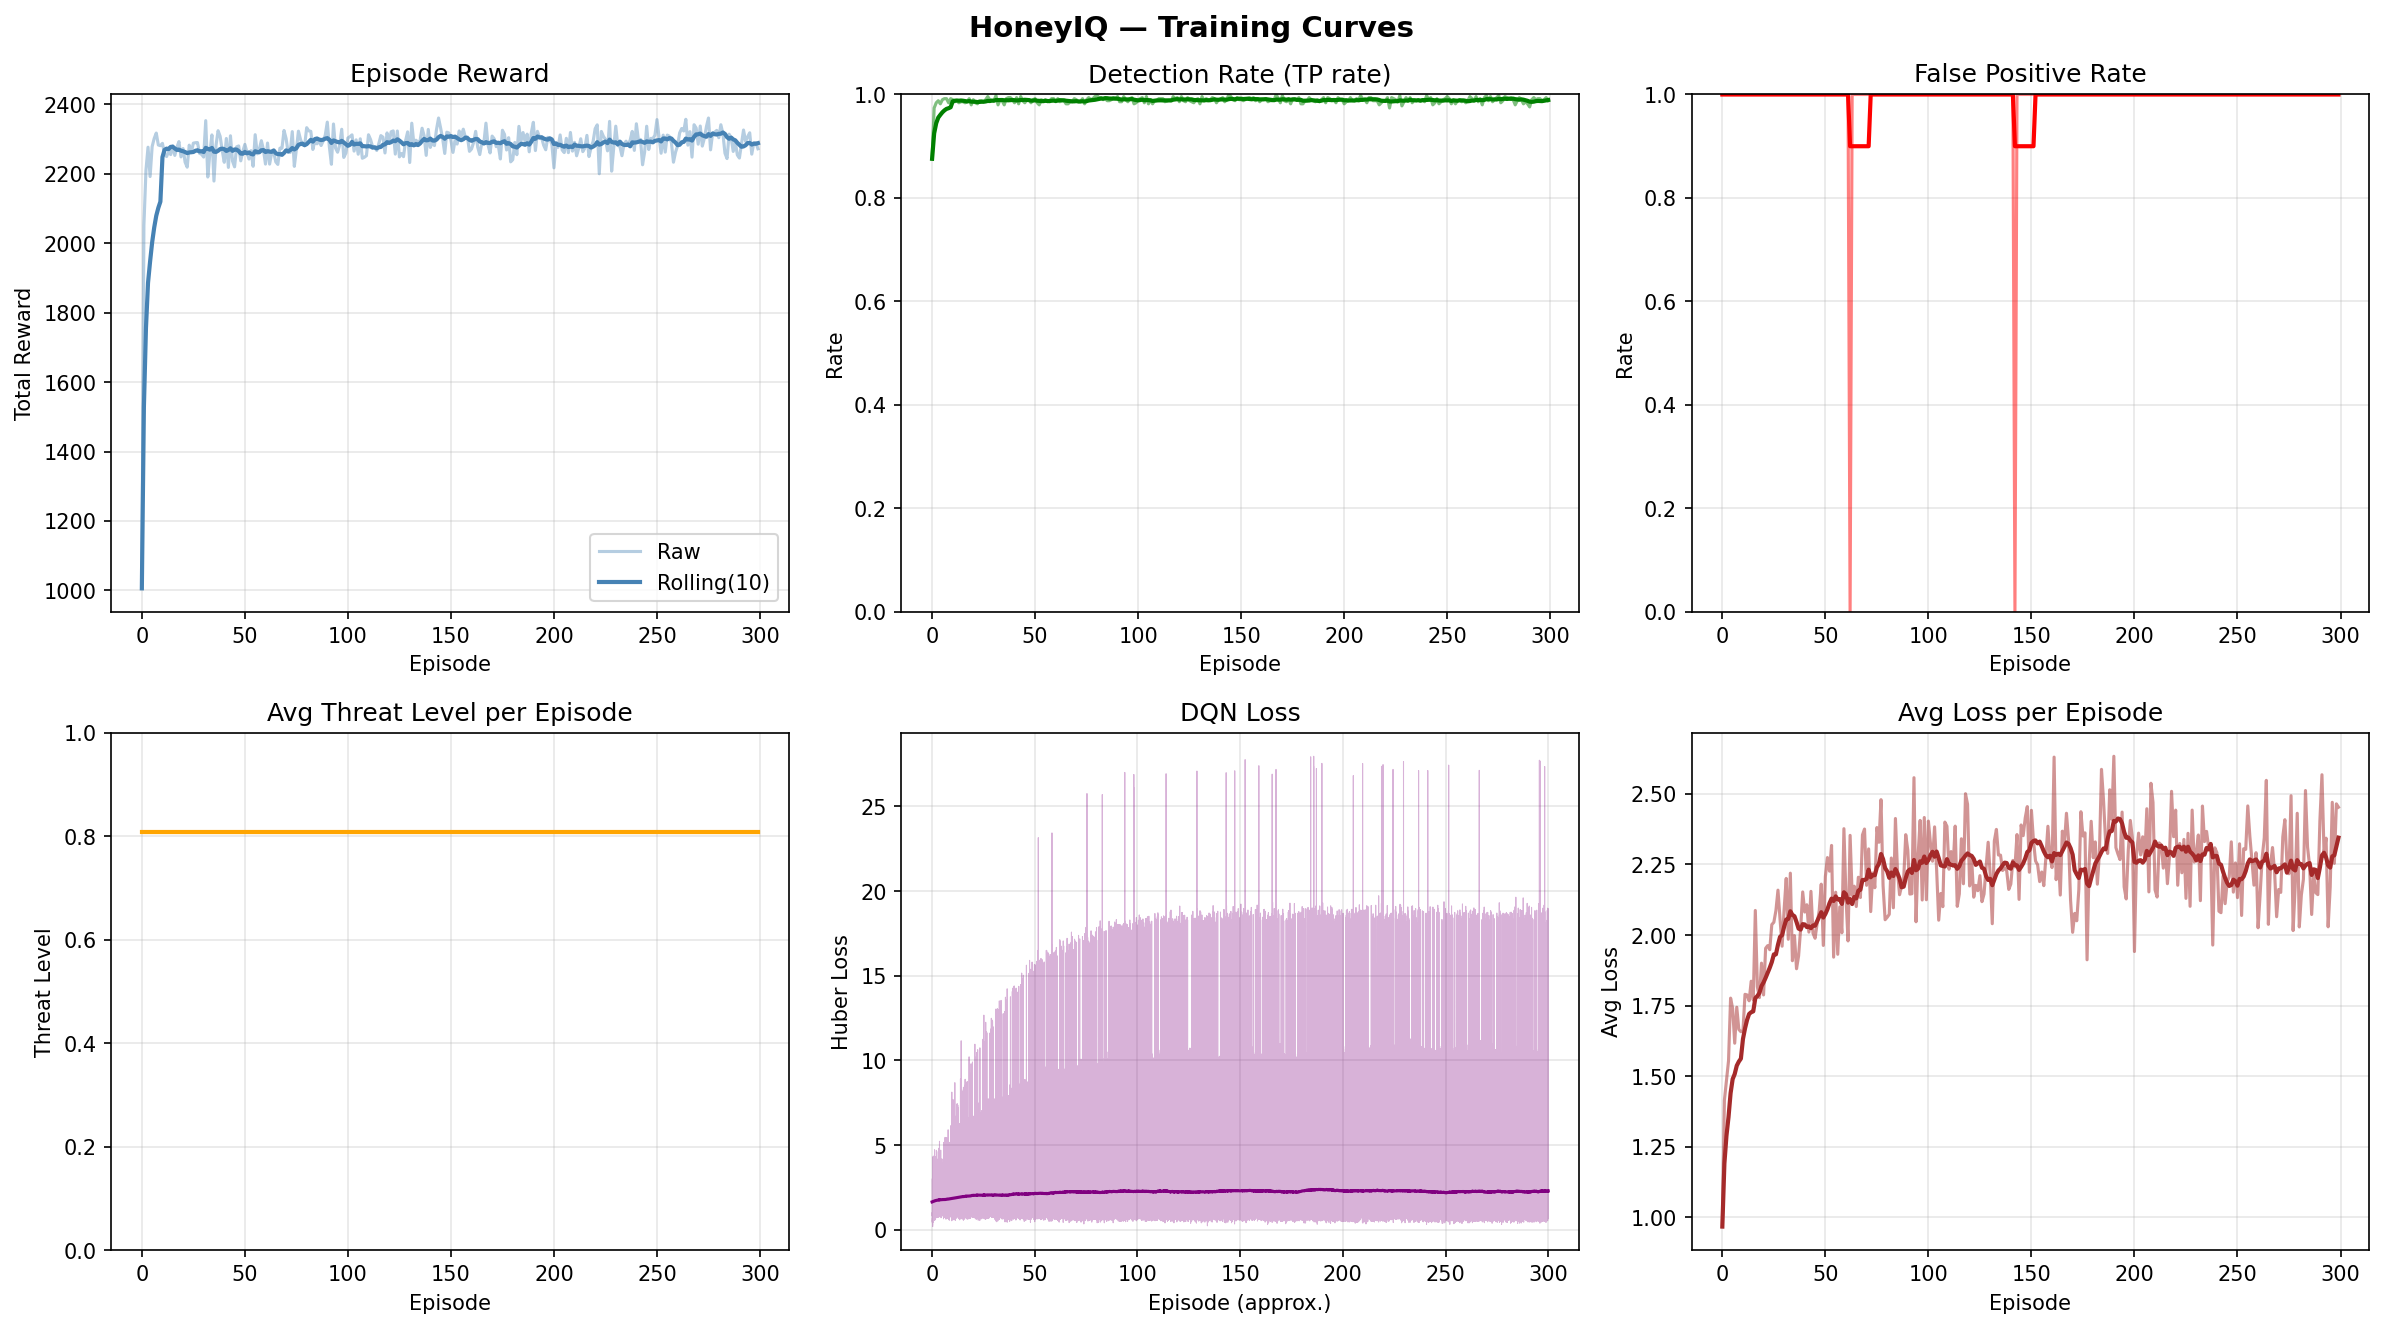
\includegraphics[width=0.92\textwidth]{figures/training_curves}
  \caption{DQN training curves over 300 episodes.
           \emph{Top row, left to right}: episode total reward (raw and
           rolling 10-episode mean); episode detection rate; episode
           false-positive rate.
           \emph{Bottom row, left to right}: average episode threat level;
           per-update Huber loss (smoothed); per-episode average loss.}
  \label{fig:training_curves}
\end{figure}

\subsection{Episode Reward}

Episode reward climbs rapidly from 1\,006 at episode~0 to approximately
2\,051 at episode~1, then continues to rise to a plateau of 2\,200--2\,360
by episode~30 (Figure~\ref{fig:training_curves}, top-left).
The dramatic improvement between episodes 0 and 1 reflects the structure of
the OPPORTUNISTIC attacker: even a partially trained policy quickly learns
that non-ALLOW actions yield positive rewards on the dense attack traffic,
causing a substantial reward increase as soon as the replay buffer contains
enough transitions for a meaningful Q-value update.

The rolling 10-episode mean stabilises at approximately 2\,300 from
episode~50 onwards, with relatively small episode-to-episode variance
($\sigma \approx 35$), indicating that the policy has converged to a
stable strategy.
The absence of reward collapse (a common failure mode in DQN training)
suggests that the target network and gradient clipping together provide
adequate stabilisation.

\subsection{Detection Rate}

Detection rate starts at 87.6\% at episode~0, rises sharply to 97.4\% at
episode~1, and exceeds 98.5\% from episode~3 onwards
(Figure~\ref{fig:training_curves}, top-centre).
The high starting detection rate (87.6\%) is consistent with the
OPPORTUNISTIC attacker's continuous attack traffic: even a random policy
that selects non-ALLOW actions for the majority of steps will detect most
attacks because the benign fraction of traffic is small.

Detection rates fluctuate within a narrow band ($98.5$--$99.5\%$) throughout
training, with occasional dips to $\approx$\,97\% corresponding to episodes
where the epsilon-greedy policy selects suboptimal ALLOW responses more
frequently than usual.

\subsection{False-Positive Rate}

The false-positive rate exhibits a distinctive pattern: it remains at
essentially 1.0 throughout most of training, with occasional drops to 0.0
at isolated episodes (e.g., episodes 62 and 142).
This bimodal behaviour reflects the fact that false positive events are
rare in the OPPORTUNISTIC scenario (the attacker generates predominantly
attack traffic), so the per-episode false-positive rate is either 1.0
(the episode happened to contain a benign step and the DQN responded
with a non-ALLOW action) or 0.0 (no benign steps occurred, making the
false positive rate undefined or effectively zero).

This finding reveals an important distinction between the DQN training
environment and the SEDM evaluation: the DQN training set is dominated
by attack traffic, providing limited signal for learning to discriminate
benign traffic.
The SEDM's explicit ALLOW entry in the matrix for Reconnaissance/Low
provides a structural guarantee that benign-like traffic at early kill
chain stages is handled correctly, without requiring the learner to observe
rare benign examples.

\subsection{DQN Training Loss}

Per-update Huber loss increases from $\approx$\,0.97 at training start
(episode~0) to $\approx$\,1.4--1.6 by episodes 1--10, then gradually
rises to $\approx$\,2.0--2.6 and stabilises with moderate variance through
episodes 50--300 (Figure~\ref{fig:training_curves}, bottom panels).

The rising loss during early training is expected: as the policy network
learns to produce larger Q-value estimates for highly rewarding actions, the
Huber targets also grow, causing the raw loss value to increase even as the
\emph{relative} TD error decreases.
The absence of large upward spikes in the later training phase indicates
that gradient clipping and the target network together prevent instability.
The persistent moderate variance in per-update loss ($\approx$\,$\pm$0.5$\sigma$
around the rolling mean) is characteristic of off-policy DQN training with a
diverse replay buffer.

\begin{table}[ht]
  \centering
  \caption{DQN training performance at selected training milestones
           (OPPORTUNISTIC intent, 500 steps per episode).}
  \label{tab:dqn_milestones}
  \begin{tabular}{rrrrrr}
    \toprule
    Episode & Total Reward & Det.\ Rate & FP Rate & Avg Threat & Avg Loss \\
    \midrule
    0   & 1\,006.0 & 87.6\% & 100.0\% & 0.808 & 0.967 \\
    1   & 2\,051.6 & 97.4\% & 100.0\% & 0.808 & 1.415 \\
    10  & 2\,288.0 & 99.0\% & 100.0\% & 0.808 & 1.661 \\
    50  & 2\,285.0 & 99.2\% & 100.0\% & 0.808 & 2.207 \\
    100 & 2\,303.5 & 99.0\% & 100.0\% & 0.808 & 2.404 \\
    150 & 2\,297.1 & 99.0\% & 100.0\% & 0.808 & 2.442 \\
    200 & 2\,217.4 & 98.2\% & 100.0\% & 0.808 & 1.942 \\
    250 & 2\,356.4 & 99.6\% & 100.0\% & 0.808 & 2.133 \\
    299 & 2\,272.4 & 98.8\% & 100.0\% & 0.808 & 2.453 \\
    \bottomrule
  \end{tabular}
\end{table}

\subsection{Comparison with SEDM}

The DQN and SEDM are compared on the metrics available from both systems.
On the OPPORTUNISTIC intent (the DQN's training distribution), the DQN
achieves detection rates of 98.5--99.6\% with training reward
2\,200--2\,360 per 500-step episode.
The SEDM achieves 99.41\% detection on OPPORTUNISTIC in 200-step evaluation
episodes.

However, the DQN's false-positive rate is effectively undefined in training
(benign steps are too rare for a meaningful estimate), while the SEDM
achieves 15.00\% on OPPORTUNISTIC in evaluation episodes that include more
diverse traffic.
The DQN requires 300 training episodes (150\,000 environment steps) to
reach its performance level; the SEDM requires no training.

The DQN's opaque Q-values provide no direct insight into why particular
actions are chosen, while the SEDM's five-step algorithm is fully
traceable to observable inputs.
This interpretability advantage is examined further in the Discussion
(Chapter~\ref{ch:discussion}).

%% ── 4.6 Metric Comparison Summary ───────────────────────────
\section{Cross-Intent Metric Comparison}
\label{sec:results_compare}

Figure~\ref{fig:metric_comparison} presents a comparative view of the four
key metrics across attacker intents.

\begin{figure}[ht]
  \centering
  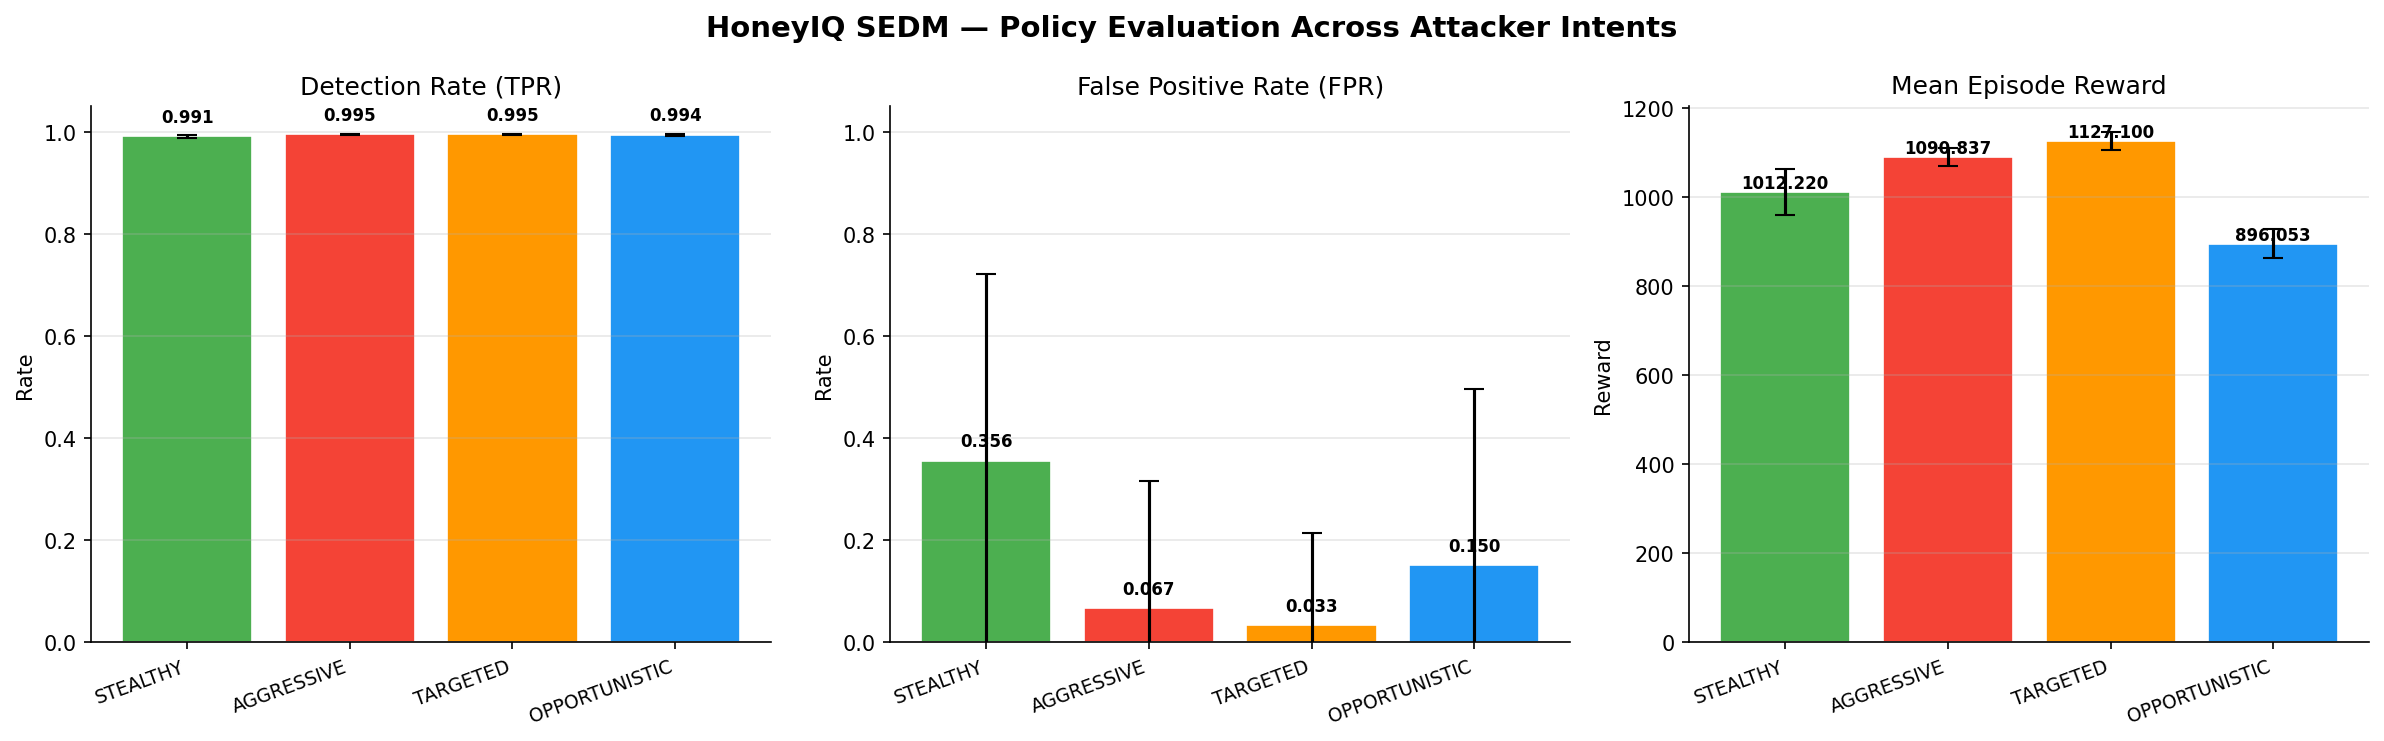
\includegraphics[width=0.88\textwidth]{figures/metric_comparison}
  \caption{Side-by-side comparison of mean reward, detection rate,
           false positive rate, and average threat level for each attacker
           intent.
           Error bars show $\pm$1 standard deviation over 30 episodes.}
  \label{fig:metric_comparison}
\end{figure}

Figure~\ref{fig:radar_comparison} shows the same metrics as a radar chart,
enabling simultaneous comparison across all four dimensions.
The radar chart reveals that TARGETED achieves the best overall balance:
highest detection rate, lowest false positive rate, and highest mean reward.
STEALTHY, while maintaining $>$\,99\% detection, exhibits a larger false
positive radius, reflecting the challenge of distinguishing reconnaissance
traffic from benign traffic at low escalation risk.

\begin{figure}[ht]
  \centering
  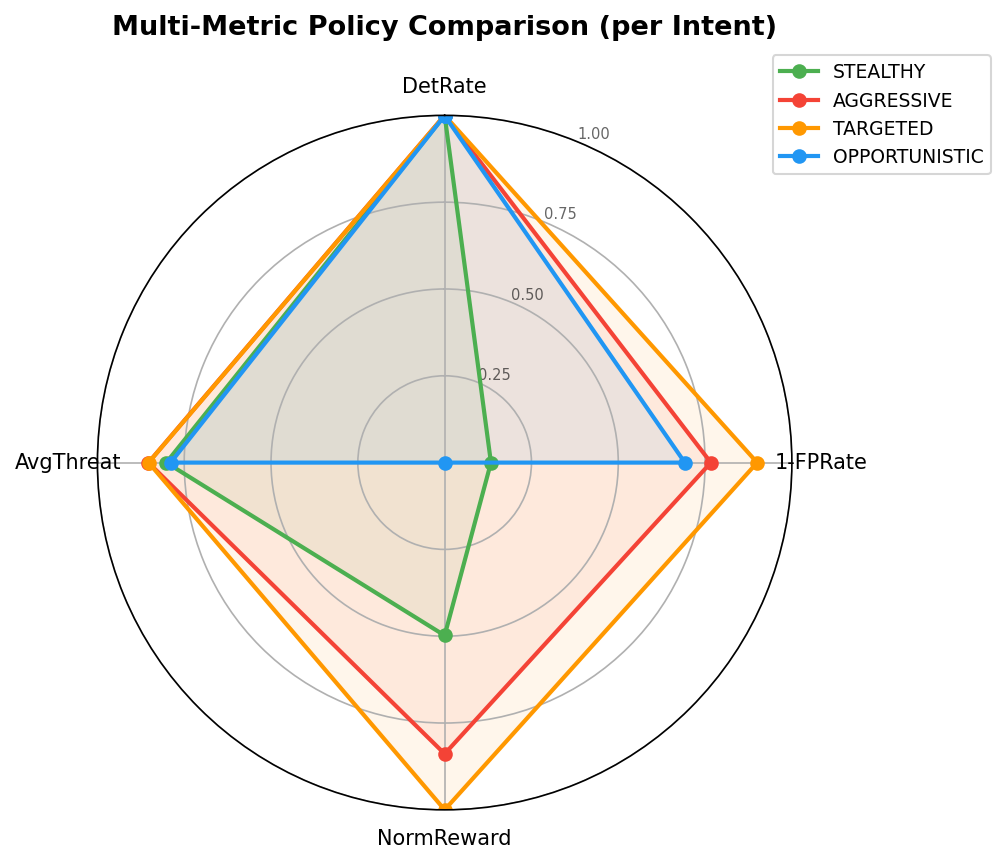
\includegraphics[width=0.70\textwidth]{figures/radar_comparison}
  \caption{Radar chart comparing SEDM performance across attacker intents
           on four normalised metrics:
           detection rate, false positive rate (inverted: lower is better),
           mean reward (normalised), and average threat level.}
  \label{fig:radar_comparison}
\end{figure}
